Considera la funció
\[
f(x)=\begin{cases}
  (x+1)^2 & \si{x\le 0},\\[4pt]
  \dfrac{1}{x-1} & \si{x>0}.
\end{cases}
\]

\begin{apartats}

\apartat[1,25]{1}
Estudia'n la continuïtat i troba'n les asímptotes.

\begin{solucio}
Cada branca és contínua al seu tros, excepte en $x=1$, que és \textbf{dins} del segon i hi anul·la el
denominador.\\
En $x=0$: $f(0)=1$ i $\lim_{x\to0^-}f(x)=1$, però $\lim_{x\to0^+}f(x)=\dfrac{1}{0-1}=-1$. Laterals finits
i diferents: \textbf{salt finit} (de salt $2$).\\
En $x=1$: la funció no hi està definida, i els laterals valen $-\infty$ (per l'esquerra) i $+\infty$
(per la dreta): \textbf{salt infinit}. La funció és contínua a $\mathbb{R}\setminus\{0,1\}$.\\
\textbf{Asímptotes}: vertical $x=1$. Per la dreta, $\lim_{x\to+\infty}f(x)=0$: asímptota horitzontal
$y=0$. Per l'esquerra, $\lim_{x\to-\infty}(x+1)^2=+\infty$: branca parabòlica, sense asímptota.
\end{solucio}

\begin{nomesllarg}
\apartat{0,75}
Estudia'n la monotonia i troba'n els extrems.

\begin{solucio}
Per a $x<0$: $f'(x)=2(x+1)$, negativa a $(-\infty,-1)$ i positiva a $(-1,0)$.\\
Per a $x>0$: $f'(x)=\dfrac{-1}{(x-1)^2}<0$: decreix a $(0,1)$ i a $(1,+\infty)$.\\
\textbf{Mínim relatiu} $(-1,0)$. En $x=0$, $f(0)=1$ és més gran que tots els valors del voltant: per
l'esquerra s'hi arriba creixent, i per la dreta la funció val prop de $-1$. És un \textbf{màxim
relatiu}, tot i que la funció no hi és contínua.
\end{solucio}
\end{nomesllarg}

\begin{tria}{trossos-tasca}
\itemtria{original}{0,75}{1,25}
Representa la funció.

\begin{solucio}
A l'esquerra, la paràbola $y=(x+1)^2$ fins al punt $(0,1)$, amb el vèrtex en $(-1,0)$. A la dreta,
les dues branques de la hipèrbola $y=\frac{1}{x-1}$: la primera surt de prop de $(0,-1)$, punt que no
és de la gràfica, i baixa cap a $-\infty$; la segona baixa des de $+\infty$ i s'acosta a l'eix $OX$.
\begin{center}
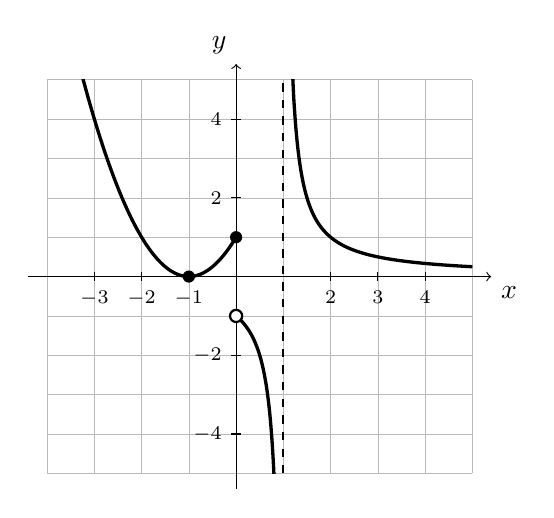
\begin{tikzpicture}[x=0.6cm,y=0.5cm]
  \draw[gray!55,very thin,step=1] (-4,-5) grid (5,5);
  \draw[->] (-4.4,0) -- (5.4,0) node[below right] {$x$};
  \draw[->] (0,-5.4) -- (0,5.4) node[above left] {$y$};
  \foreach \i in {-3,-2,-1,2,3,4} \draw (\i,0.12) -- (\i,-0.12) node[below,font=\scriptsize] {$\i$};
  \foreach \j in {-4,-2,2,4} \draw (0.1,\j) -- (-0.1,\j) node[left,font=\scriptsize] {$\j$};
  \draw[dashed,thick] (1,-5) -- (1,5);
  \begin{scope}
    \clip (-4,-5) rectangle (5,5);
    \draw[\colorgrafica,very thick,domain=-3.4:0,samples=80,smooth] plot (\x,{(\x+1)*(\x+1)});
    \draw[\colorgrafica,very thick,domain=0:0.83,samples=80,smooth] plot (\x,{1/(\x-1)});
    \draw[\colorgrafica,very thick,domain=1.17:5,samples=80,smooth] plot (\x,{1/(\x-1)});
  \end{scope}
  \fill (0,1) circle (2.2pt); \fill (-1,0) circle (2.2pt);
  \draw[fill=white,thick] (0,-1) circle (2.2pt);
\end{tikzpicture}
\end{center}
\end{solucio}

\itemtria{recorregut}{0,75}{1,25}
Troba el recorregut de $f$. Hi ha cap valor de $k$ per al qual l'equació $f(x)=k$ no tingui cap
solució?

\begin{solucio}
Per a $x\le0$, la paràbola baixa des de $+\infty$ fins al vèrtex, $(-1,0)$, i puja fins a $f(0)=1$:
hi pren tots els valors de $[0,+\infty)$.\\
A $(0,1)$, $\dfrac{1}{x-1}$ decreix des de prop de $-1$ fins a $-\infty$: hi pren els de
$(-\infty,-1)$. El valor $-1$ no s'assoleix, perquè $\dfrac{1}{x-1}=-1$ només si $x=0$, que és de
l'altra branca.\\
A $(1,+\infty)$, decreix des de $+\infty$ i s'acosta a $0$ sense arribar-hi: hi pren els de
$(0,+\infty)$.\\
Recorregut: $(-\infty,-1)\cup[0,+\infty)$. L'equació $f(x)=k$ \textbf{no té cap solució} si
$-1\le k<0$.
\end{solucio}
\end{tria}

\end{apartats}
